\subsection{Map}
The map shows the status of the countries on Earth at this certain moment of history set in the timeline -- the \textbf{NowDate}. For this project we used a self-made dataset of historic countries of whole Europe from 1945 until today and from Western, Northern, Southern and Central Europe from 1871 until 1945. We organized the data in a way that we can visualize historic changes of countries on the map. Finally we provided a funtionality to style the areas due to a current theme, for example all countries belonging to NATO at the NowDate get a blue background color.

\subsubsection{Historic Countries} % (fold)
\label{ssub:historic_countries}

A country consists of a \textbf{geometry}, represented as a multipolygon in a geojson file, a \textbf{label} with the name and the position of the country and a set of historic \textbf{changes} stating at what date geometries and labels of countries have changed.

\paragraph{Geometry} % (fold)
% paragraph geometry (end)
Everything is based on a dataset of the current countries in Europe from \textit{Natural Earth Data}
\footnote{1:10m Cultural Vectors | \url{http://www.naturalearthdata.com/downloads/10m-cultural-vectors/}}.
We extracted only the countries of Europe and loaded them into \textit{QuantumGIS}, an open source GIS software for organizing, analyzing and visualizing geometry on Earth. For each historic country we found an historic map online and created the geometry of the country using the \textit{Vector Geoprocessing Tools} of QuantumGIS. In \ref{fig:qgis} you can see the geometries of Germany from 1871 until today, from light green to dark green: The German Reich from 1871 until 1919, Weimar Republic and Third Reich after Treaty of Versailles from 1919 until 1945, reunified Germany after 1990 and the GDR from 1949 until 1990 without West Berlin.

\begin{figure}[H]
  \begin{center}
    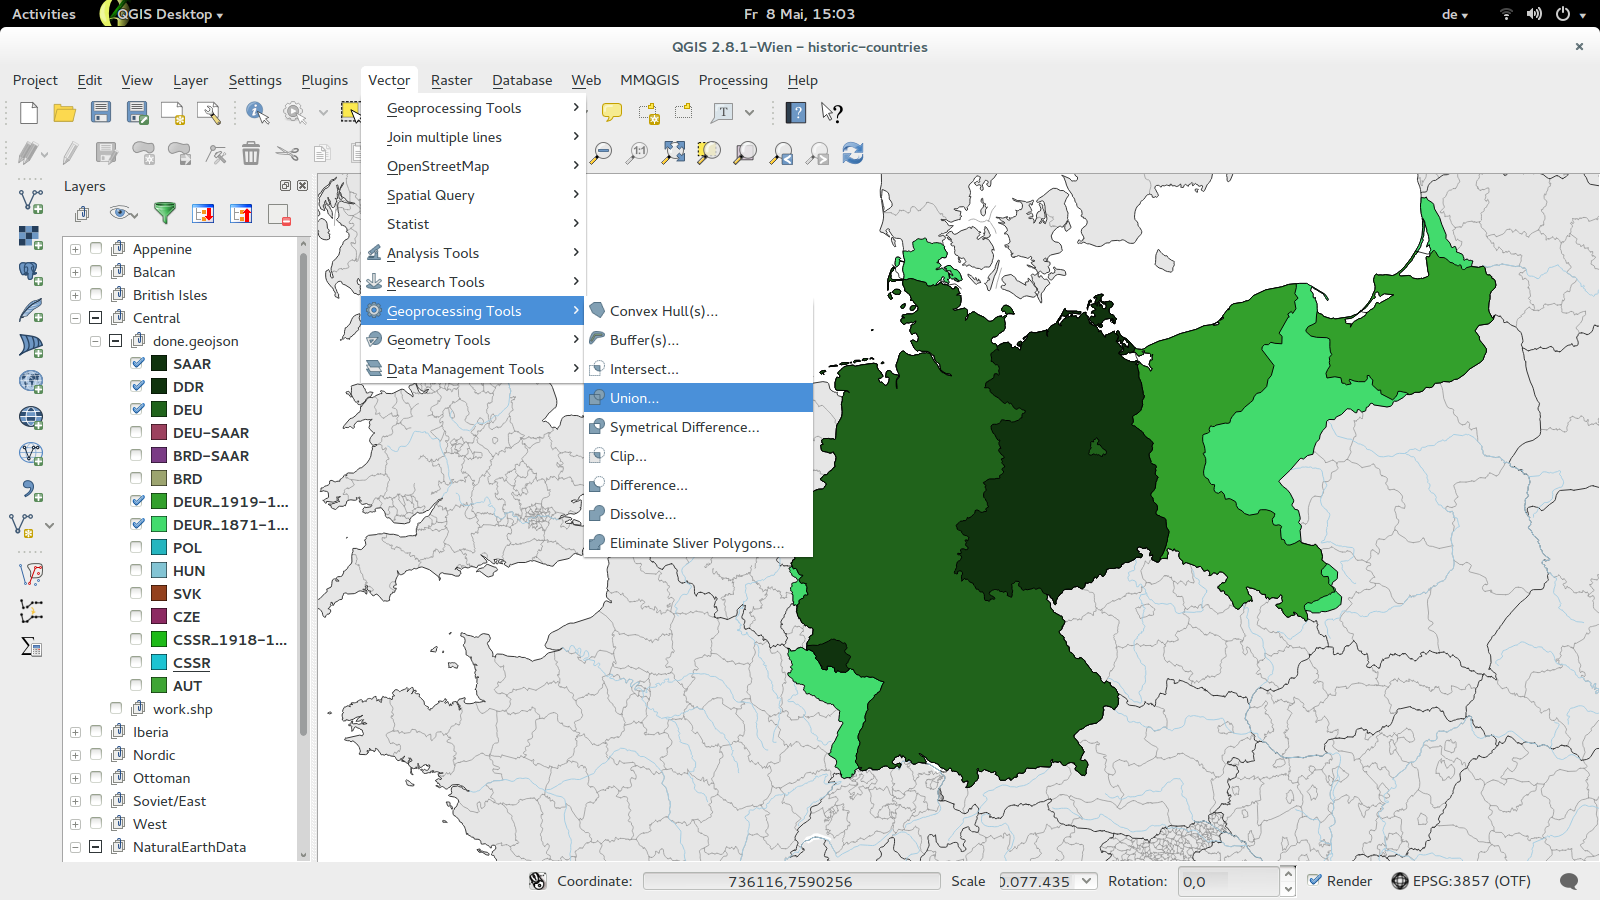
\includegraphics[width=0.9\textwidth]{graphics/qgis.png}
  \end{center}
  \caption{Geometry Manipulation of Historic Countries in QuantumGIS}
  \label{fig:qgis}
\end{figure}
\label{par:geometry}

\paragraph{Labels} % (fold)
\label{par:labels}

% paragraph labels (end)

\paragraph{Changes} % (fold)
\label{par:changes}

% paragraph changes (end)

Because of the very problematic Usability of QuantumGIS and the mass of data that would have needed to be processed we have not reached the goal to create a data base of all historic countries in Europe from 1871 on, but only from 1945 on, due to the time constraint.

% subsubsection historic_countries (end)

\subsubsection{Architecture of Historic Changes} % (fold)
\label{ssub:architecture_of_historic_changes}
separated the countries areas and labels and


\begin{figure}[H]
  \begin{center}
    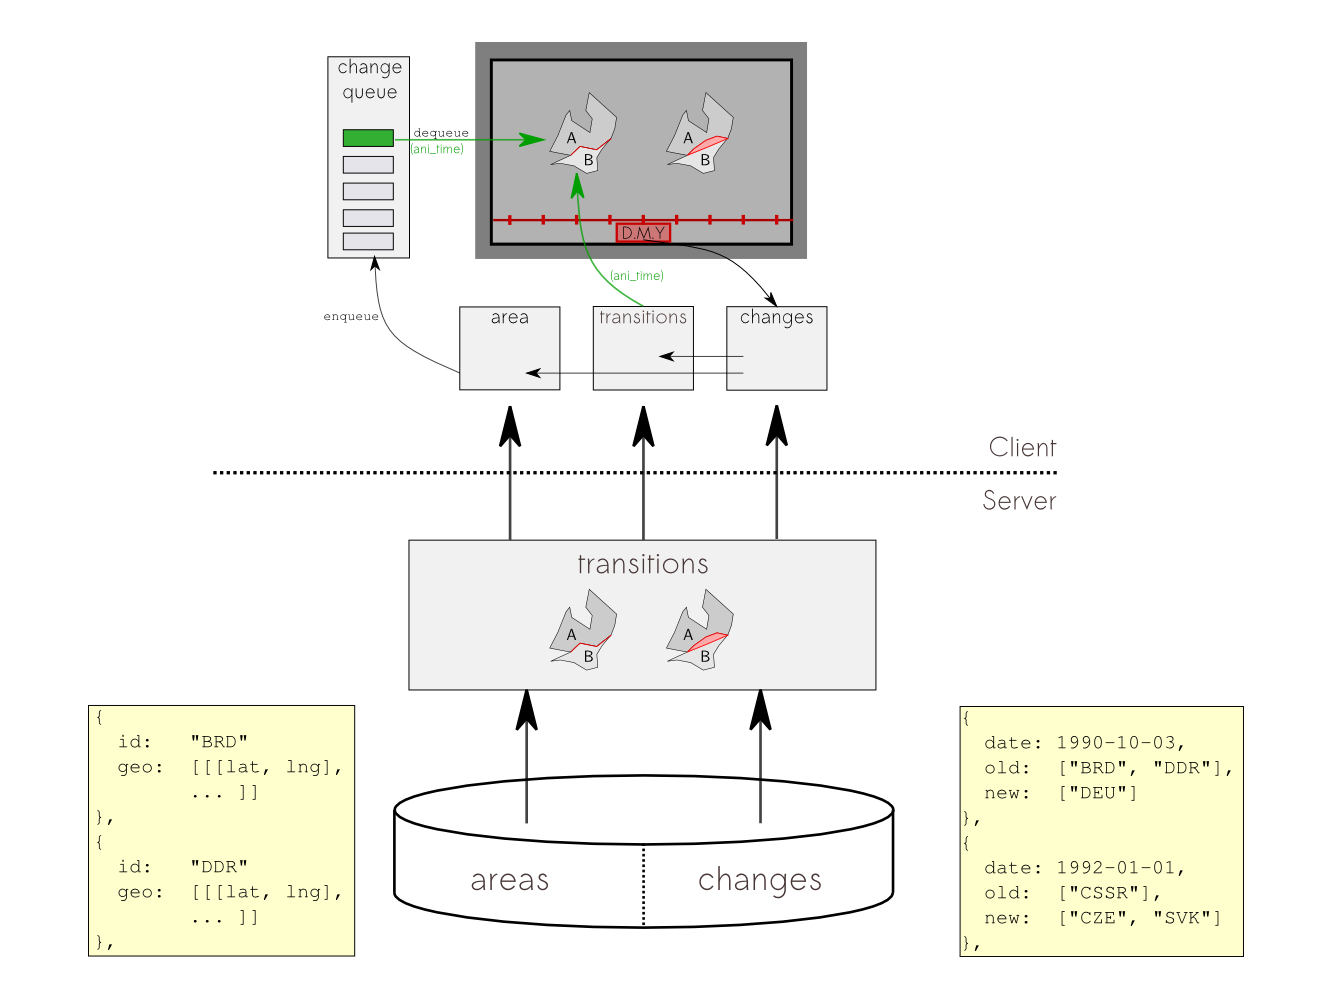
\includegraphics[width=0.9\textwidth]{graphics/historic_countries.png}
  \end{center}
  \caption{Architecture of historic countries on the map}
  \label{fig:figure1}
\end{figure}
% subsubsection architecture_of_historic_changes (end)

\subsubsection{Styling the Countries} % (fold)
\label{ssub:styling_the_countries}

% subsubsection styling_the_countries (end)

